%%%%%%%%%%%%%%%%%%%%%%%%%%%%%%%%%%%%%%%%%%
% Engineering problems / LaTeX Template
%		Semester 5
%		Institut d'Optique Graduate School
%%%%%%%%%%%%%%%%%%%%%%%%%%%%%%%%%%%%%%%%%%
%	5N-ONIP-Block1	/ Python for Science
%%%%%%%%%%%%%%%%%%%%%%%%%%%%%%%%%%%%%%%%%%
%
% Created by:
%	Julien VILLEMEJANE - 23/may/2024
% Modified by:
%	
%
%%%%%%%%%%%%%%%%%%%%%%%%%%%%%%%%%%%%%%%%%%
% Professional Newsletter Template
% LaTeX Template
% Version 1.0 (09/03/14)
%
% Created by:
% Bob Kerstetter (https://www.tug.org/texshowcase/) and extensively modified by:
% Vel (vel@latextemplates.com)
% 
% This template has been downloaded from:
% http://www.LaTeXTemplates.com
%
% License:
% CC BY-NC-SA 3.0 (http://creativecommons.org/licenses/by-nc-sa/3.0/)
%
%%%%%%%%%%%%%%%%%%%%%%%%%%%%%%%%%%%%%%%%%

\documentclass[a4paper,11pt]{article} % The default font size is 10pt; 11pt and 12pt are alternatives


\usepackage{opto_elec_villemejane}


%%%%%%%%%%%%%%%%%%%%%%%%%%%%%%%%%%%%%%%%%%%%%%%%
%%%%%%%%%%%%%%%%%%%%%%%%%%%%%%%%%%%%%%%%%%%%%%%%
%%%%%%%%%%%%%%%%%%%%%%%%%%%%%%%%%%%%%%%%%%%%%%%%
%%%%%%%%%%%%%%%%%%%%%%%%%%%%%%%%%%%%%%%%%%%%%%%%
\begin{document}
\newpage
\pagestyle{empty}

\begin{minipage}[c]{.25\linewidth}
	
\includegraphics[width=4cm]{images/Logo-LEnsE.png}
\end{minipage} \hfill
\begin{minipage}[c]{.4\linewidth}

\begin{center}
\vspace{0.3cm}
{\Large OPTO-ELECTRONIQUE}

\medskip

\textbf{\Large TP Introduction}

\end{center}
\end{minipage}\hfill

\begin{center}
\vspace{0.3cm}

\noindent \rule{\linewidth}{1pt}

Durée : 3h / Découverte de la photodétection / Capteur de luminosité

\vspace{-0.2cm}
\noindent \rule{\linewidth}{1pt}
\end{center}

%%%%%%%%%%%%%%%%%%%%%%%%%%%%%%%%%%
\section*{Objectifs de l'expérience}

L'objectif du TP est de réaliser un \textbf{éclairage adaptatif} en fonction de la luminosité de l'environnement mesurée grâce à un \textbf{capteur de type photodiode}.

Cette séance a également pour but de vous familiariser avec l'utilisation des appareils de mesure mis à votre disposition au cours des séances de Travaux Pratiques d'Opto-Electronique.


%%%%%%%%%%%%%%%%%%%%%%%%%%%%%%%%%%
%%%%%%%%%%%%%%%%%%%%%%%%%%%%%%%%%%
%%%%%%%%%%%%%%%%%%%%%%%%%%%%%%%%%%
\section{PARTIE A - Capteur de luminosité}

On s'intéresse au montage suivant avec $E = 5 \, V$ et $R_{PHD} = 100 \, k\Omega$:

\begin{center}
\begin{circuitikz}
	\draw (0,0) to[battery2, invert] (0,3) -- (2,3);
	% fleche
	\draw (-0.5,0.3) edge[->] (-0.5,2.7);
	\node (Ein) at (-1,1.5){$E$};
	
	\draw (5,3) to[empty photodiode] (2,3);
	\draw (2,3) to[short, i = $I_{photo}$, current arrow scale=8] ++(0.5,0);

	\draw (5,3) to[R=$R_{PHD}$, *-*] (5,0) -- (0,0);
	\draw (5,0) to[short, -o] ++(1.5,0);
	\draw (5,3) to[short, -o] ++(1.5,0);
	\draw (5,0) node[ground](GND){};
	% fleche
	\draw (6.5,0.3) edge[->, green!40!black] (6.5,2.7); 
	\node[text=green!40!black] (US) at (7.1,1.5){$V_S$};
\end{circuitikz}
\end{center}

Une photodiode est un composant électronique fournissant un courant d'intensité proportionnelle à la valeur de l'éclairement appliquée sur celle-ci. Les caractéristiques de la photodiode étudiée (\textit{SFH206K}) sont fournies ci-dessous:
	\begin{center}
		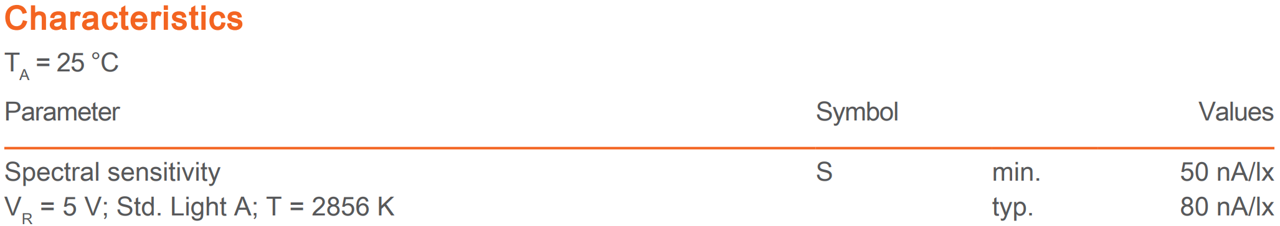
\includegraphics[width=15cm]{images/Photodiode.png}
	\end{center}

\subsection*{A1 - Etude du capteur}

\Real Mesurer l'éclairement moyen de la salle à l'aide d'un luxmètre. Estimer la valeur de la tension qui apparaitra aux bornes de la résistance $R_{PHD}$ lorsque le circuit est alimenté avec une tension $E = 5 \,V$.

\Real Câbler le montage ci-dessus et mettre en place une mesure de la tension aux bornes de $R_{PHD}$. 

\Real Visualiser la tension aux bornes de $R_{PHD}$ à l'aide d'un oscilloscope et comparer le signal observé au signal attendu.

\newpage
\subsection*{A2 - Mise en forme du signal}

\begin{multicols}{2}

On se propose d'utiliser le montage suivant pour supprimer les composantes fréquentielles non souhaitées. \textit{Tous les potentiels sont référencés par rapport à la masse.}

La fonction de transfert de ce montage est la suivante : 

$$\frac{V_s}{V_e} = -\frac{R_2}{R_1} \cdot \frac{1}{1 + j\cdot R_2 \cdot C \cdot \omega}$$

\medskip

\Real Quelle fréquence de coupure choisir pour répondre au cahier des charges ?

\columnbreak

\begin{center}
\begin{circuitikz} 
	\node [op amp, fill=blue!10!white](A1) at (0,0){\texttt{ALI1}};
	\draw (A1.-) to[short] ++(-.5,0) coordinate(A) to[short, -*] ++(0,1.5) coordinate(B) to[R, l^=$R_2$] (B -| A1.out) coordinate(RR) to[short, *-*] (A1.out);
	\draw (B) -- ++(0, 1.5) coordinate(CC) to[C, l^=$C$] (CC -| A1.out) -- (RR);  
	\draw (A1.-) to[short,-*] ++(-.5,0) coordinate(AA) to[R, l_=$R_1$] ++(-2.5,0) coordinate(BB) to [short,l_=${V_e}$, -o] ++(-1,0) coordinate(CC);


	\draw (A1.+) to[short] ++(-.5,0) coordinate(AA2) node[cground]{};

	\draw (A1.out) to [short,l=${V_S}$, -o] ++(1,0) coordinate(D);
	
\end{circuitikz}
\end{center}
\end{multicols}


\Real Câbler ce montage et faire une étude fréquentielle de son fonctionnement pour confirmer qu'il réalise bien la fonction souhaitée. \textit{L'ALI sera alimenté à l'aide d'une alimentation symétrique de +/- 5V.}

\Real Cascader alors le capteur de luminosité avec le circuit proposé et conclure quant à l'amélioration effective du signal. Ajuster le montage si nécessaire

%%%%%%%%%%%%%%%%%%%%%%%%%%%%%%%%%%
%%%%%%%%%%%%%%%%%%%%%%%%%%%%%%%%%%
%%%%%%%%%%%%%%%%%%%%%%%%%%%%%%%%%%

\section{PARTIE B - Comparateur}


\begin{multicols}{2}

On souhaite caractériser 3 niveaux de luminosité spécifiques qui amèneront à l'adaptation de l'éclairage de l'environnement. Pour cela, on propose le circuit suivant à connecter directement en sortie des montages précédents.

\Real Expliquer le principe de fonctionnement de ce montage.

\Real Proposer un montage simple (et visuel) à placer en sortie des amplificateurs linéaires afin de pouvoir visualiser le fonctionnement du système.

\Real Câbler le montage en proposant une valeur pertinente pour $U_{ref}$. On prendra $R_1 = R_2 = R_3 = 3.3\operatorname{k\Omega}$. Vérifier le bon fonctionnement de ce circuit.

\Real Cascader alors l'ensemble des circuits afin d'obtenir le système complet et vérifier son bon fonctionnement, notamment lorsque le capteur de luminosité est placé dans l'ombre.


\columnbreak

\begin{center}
\begin{circuitikz} 
	\node [op amp, fill=blue!10!white](A1) at (0,2.2){\texttt{ALI2}};
	\node [op amp, fill=blue!10!white](A2) at (0,0){\texttt{ALI3}};
	% Input	
	\draw (A1.+) to[short,-*] ++(-.5,0) coordinate(A1A);
	\draw (A2.+) -- ++(-.5,0) coordinate(A2A);
	\draw (A1A) -- (A2A);
	\draw (A1A) -- ++(0, 4) to[short,-o] ++(-5, 0) coordinate(UIN);
	\draw[->, red] (GND -| UIN) -- ($(UIN) + (0,-0.5)$);

	% Divider
	\draw (A1.-) to[short,-*] ++(-1.5,0) coordinate(A1B);
	\draw (A2.-) to[short,-*] ++(-1.5,0) coordinate(A2B);
	\draw (A1B) to[R, l_=$R_2$] (A2B);
	\draw (A2B) to[R, l_=$R_3$] ++(0,-2) coordinate(GND) node[cground]{};
	\draw (A1B) to[R, l^=$R_1$] ++(0,+2) to[short,-o] ++(-2,0) coordinate(UREF);
	
	% Outputs
	\draw (A1.out) to[short,-o] ++(0.5,0) coordinate(A1O);
	\draw (A2.out) to[short,-o] ++(0.5,0) coordinate(A2O);

	\draw[->, blue] (GND -| UREF) -- ($(UREF) + (0,-0.5)$);
	\node[text={blue}] (Vref) at ($(UREF) + (-0.5,-2.5)$){$V_{REF}$}; 
	\node[text={red}] (Vin) at ($(UIN) + (-0.5,-2.5)$){$V_{E}$}; 
	
\end{circuitikz}
\end{center}

\end{multicols}



%%%%%%%%%%%%%%%%%%%%%%%%%%%%%%%%%%
%%%%%%%%%%%%%%%%%%%%%%%%%%%%%%%%%%
%%%%%%%%%%%%%%%%%%%%%%%%%%%%%%%%%%
\section{LIVRABLES}

Vous devez pour chaque expérience proposée dans ce sujet :

\begin{itemize}
	\item Rédiger le protocole de mesure utilisé, incluant le paramétrage des différents instruments de mesure.
	\item Reporter les mesures effectués et réaliser des captures d'oscilloscope de signaux pertinents.
	\item Analyser les résultats et comparer aux attentes prévues.
\end{itemize}

%%%%%%%%%%%%%%%%%%%%%%%%%%%%%%%%%%%%%%%%%%%%%%%%%%%%%%%%%%%%%%%%%%%%%%%%%%%%%%%%%%%%%
\end{document}
